\documentclass[journal,12pt,twocolumn]{IEEEtran}

\usepackage{setspace}
\usepackage{gensymb}

\singlespacing


\usepackage[cmex10]{amsmath}

\usepackage{amsthm}

\usepackage{mathrsfs}
\usepackage{txfonts}
\usepackage{stfloats}
\usepackage{bm}
\usepackage{cite}
\usepackage{cases}
\usepackage{subfig}

\usepackage{longtable}
\usepackage{multirow}

\usepackage{enumitem}
\usepackage{mathtools}
\usepackage{steinmetz}
\usepackage{tikz}
\usepackage{circuitikz}
\usepackage{verbatim}
\usepackage{tfrupee}
\usepackage[breaklinks=true]{hyperref}
\usepackage{graphicx}
\usepackage{tkz-euclide}
\usepackage{float}

\usetikzlibrary{calc,math}
\usepackage{listings}
    \usepackage{color}                                            %%
    \usepackage{array}                                            %%
    \usepackage{longtable}                                        %%
    \usepackage{calc}                                             %%
    \usepackage{multirow}                                         %%
    \usepackage{hhline}                                           %%
    \usepackage{ifthen}                                           %%
    \usepackage{lscape}     
\usepackage{multicol}
\usepackage{chngcntr}

\DeclareMathOperator*{\Res}{Res}

\renewcommand\thesection{\arabic{section}}
\renewcommand\thesubsection{\thesection.\arabic{subsection}}
\renewcommand\thesubsubsection{\thesubsection.\arabic{subsubsection}}

\renewcommand\thesectiondis{\arabic{section}}
\renewcommand\thesubsectiondis{\thesectiondis.\arabic{subsection}}
\renewcommand\thesubsubsectiondis{\thesubsectiondis.\arabic{subsubsection}}


\hyphenation{op-tical net-works semi-conduc-tor}
\def\inputGnumericTable{}                                 %%

\lstset{
%language=C,
frame=single, 
breaklines=true,
columns=fullflexible
}
\begin{document}
\newtheorem{theorem}{Theorem}[section]
\newtheorem{problem}{Problem}
\newtheorem{proposition}{Proposition}[section]
\newtheorem{lemma}{Lemma}[section]
\newtheorem{corollary}[theorem]{Corollary}
\newtheorem{example}{Example}[section]
\newtheorem{definition}[problem]{Definition}

\newcommand{\BEQA}{\begin{eqnarray}}
\newcommand{\EEQA}{\end{eqnarray}}
\newcommand{\define}{\stackrel{\triangle}{=}}
\bibliographystyle{IEEEtran}
\providecommand{\mbf}{\mathbf}
\providecommand{\pr}[1]{\ensuremath{\Pr\left(#1\right)}}
\providecommand{\qfunc}[1]{\ensuremath{Q\left(#1\right)}}
\providecommand{\sbrak}[1]{\ensuremath{{}\left[#1\right]}}
\providecommand{\lsbrak}[1]{\ensuremath{{}\left[#1\right.}}
\providecommand{\rsbrak}[1]{\ensuremath{{}\left.#1\right]}}
\providecommand{\brak}[1]{\ensuremath{\left(#1\right)}}
\providecommand{\lbrak}[1]{\ensuremath{\left(#1\right.}}
\providecommand{\rbrak}[1]{\ensuremath{\left.#1\right)}}
\providecommand{\cbrak}[1]{\ensuremath{\left\{#1\right\}}}
\providecommand{\lcbrak}[1]{\ensuremath{\left\{#1\right.}}
\providecommand{\rcbrak}[1]{\ensuremath{\left.#1\right\}}}
\theoremstyle{remark}
\newtheorem{rem}{Remark}
\newcommand{\sgn}{\mathop{\mathrm{sgn}}}
\providecommand{\abs}[1]{\left\vert#1\right\vert}
\providecommand{\res}[1]{\Res\displaylimits_{#1}} 
\providecommand{\norm}[1]{\left\lVert#1\right\rVert}
%\providecommand{\norm}[1]{\lVert#1\rVert}
\providecommand{\mtx}[1]{\mathbf{#1}}
\providecommand{\mean}[1]{E\left[ #1 \right]}
\providecommand{\fourier}{\overset{\mathcal{F}}{ \rightleftharpoons}}
%\providecommand{\hilbert}{\overset{\mathcal{H}}{ \rightleftharpoons}}
\providecommand{\system}{\overset{\mathcal{H}}{ \longleftrightarrow}}
	%\newcommand{\solution}[2]{\textbf{Solution:}{#1}}
\newcommand{\solution}{\noindent \textbf{Solution: }}
\newcommand{\cosec}{\,\text{cosec}\,}
\providecommand{\dec}[2]{\ensuremath{\overset{#1}{\underset{#2}{\gtrless}}}}
\newcommand{\myvec}[1]{\ensuremath{\begin{pmatrix}#1\end{pmatrix}}}
\newcommand{\mydet}[1]{\ensuremath{\begin{vmatrix}#1\end{vmatrix}}}
\numberwithin{equation}{subsection}
\makeatletter
\@addtoreset{figure}{problem}
\makeatother
\let\StandardTheFigure\thefigure
\let\vec\mathbf
\renewcommand{\thefigure}{\theproblem}
\def\putbox#1#2#3{\makebox[0in][l]{\makebox[#1][l]{}\raisebox{\baselineskip}[0in][0in]{\raisebox{#2}[0in][0in]{#3}}}}
     \def\rightbox#1{\makebox[0in][r]{#1}}
     \def\centbox#1{\makebox[0in]{#1}}
     \def\topbox#1{\raisebox{-\baselineskip}[0in][0in]{#1}}
     \def\midbox#1{\raisebox{-0.5\baselineskip}[0in][0in]{#1}}
\vspace{3cm}
\title{ASSIGNMENT 3}
\author{Y.Nagarani}
\maketitle
\newpage
\bigskip
\renewcommand{\thefigure}{\theenumi}
\renewcommand{\thetable}{\theenumi}
Download all python codes from 
\begin{lstlisting}
https://github.com/Y.Nagarani/ASSIGNMENT2/tree/main/CODES
\end{lstlisting}
%
and latex-tikz codes from 
%
\begin{lstlisting}
https://github.com/Y.Nagarani/ASSIGNMENT2/tree/main
\end{lstlisting}
%
\section{Question No 2.32}
Find the shortest distance between lines 
\begin{align}
\vec{L_1}:  \vec{x} = \myvec{1 \\ 2 \\ 1} + \lambda_1\myvec{1 \\ -1 \\ 1}
\end{align}
\begin{align}
\vec{L_2}:  \vec{x} = \myvec{2 \\ -1 \\ -1} + \lambda_2\myvec{2 \\ 1 \\ 2}
\end{align}
\section{SOLUTION}  
\begin{align}
Let,
\vec{A_1} = \myvec{1 \\ 2 \\ 1} , \vec{m_1} = \myvec{1 \\ -1 \\ 1}
\end{align}
\begin{align}
\vec{A_2} = \myvec{2 \\ -1 \\ -1} , \vec{m_2} = \myvec{2 \\ 1 \\ 2}
\end{align}
The lines will interest if 
\begin{align}
\myvec{1 \\ 2 \\ 1} + \lambda_1\myvec{1 \\ -1 \\ 1} = \myvec{2 \\ -1 \\ -1} + \lambda_2\myvec{2 \\ 1 \\ 2}
\end{align}
\begin{align}
\myvec{1 & 2\\ -1 & 1 \\ 1 & 2}\myvec{\lambda_1 \\ \lambda_2} = \myvec{1 \\ -3  \\ -2 }
\end{align}
The augmented matrix for the above equation is row reduced form
\begin{align}
\myvec{1 & 2 & 1\\-1 & 1 & -3 \\ 1 & 2 & 2} 
\xleftrightarrow {R_2\leftarrow R_2 +R_1}\myvec{1 & 2 & 1 & \\0 & 3 & -2 \\1 & 2 & 2 }
\end{align}
\begin{align}
\xleftrightarrow {R_3\leftarrow R_3 - R_1}\myvec{1 & 2 & 1 \\ 0 & 3 & -2 \\ 0 & 0 & 1}
\end{align}
$\therefore$ The above matrix has rank=3. Hence the line do not interest. Given lines are not parallel but they lie on parallel planes. such lines are known as skew lines.
\\
$\therefore$ the distance between given two lines are
\begin{align}
\frac{\abs{\vec{n}^T(\vec{A_2}-\vec{A_1})}}{\norm{\vec{n}}} = \frac{\abs{(\vec{A_2}-\vec{A_1})^T(\vec{m_1} \times \vec{ m_2})}}{\norm{\vec{m_1} \times \vec{m_2}}}
\end{align}
Distance between given two lines is 4.5
\begin{figure}[!ht]
\centering
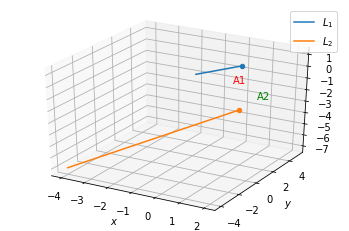
\includegraphics[width=\columnwidth]{download (7).png}
\caption{Skew Lines}
\label{fig: Skew Lines}	
\end{figure}
\end{document}